\section{ Self Adaptive R-A*mbush: Ambush with adaptive radius R}

\rambush\  provides a solution that is not as general as the one for
 \ambush.  Using the same distance $R$ for the fixed radius 
 in different maps, would produce good results in some of them 
 and bad ones in others. This means the user would have to manually 
 fix the measure of $R$ by tacking into consideration the size of 
 the map, the path cost function, or the number of obstacles. 
 In addition, given that  the cost function can be different for each 
 agent, the radius should be established according to the 
 $\lambda$ measure of every agent.
  
Thus, \sarambush\ is proposed as a variation of \rambush\ that 
solves this generality problem. Initially, This method makes each
 agent calculate the path with \astar. Then, a set of points from
  that route is chosen.  This will  be the set of the possible radius 
  $R$. The algorithm will select the minimum radius that generates 
  the greatest $\Phi$, starting from the smallest $R$.  
  This is based on the idea of starting to use sub-optimal 
  paths as late as possible.  Note that \astar\ is the specific 
  case where $R=0$ and \ambush\ is the one where $R$ is greater 
  than or equal to the real distance between the agent and the goal.  

If points that are too close to the goal are inside the set of radius, 
in particular, $R=0$, all the other agents will choose the optimal path, 
once the maximum ambush is reached. This could make the 
distribution of the agents around the goal very unbalanced towards 
the nodes that are closest to the agents stating points.

Figure \ref{unbalanced} Shows a situation where the agents distribution 
is not desirable, but the maximum ambush rate is obtained.	The agents 
colored in black performed the method \sarambush\ first. Then, the agents
in gray chose the optimal path because the ambush measure cannot 
be improved anymore, creating an unbalanced distribution around the
goal. This can be solved by taking into account a measure
 of distribution when choosing the radius. Thus, let 

\begin{equation}
  \Delta = 1-\dfrac{(\Sigma i |  i \in V 
  						\wedge i \in pred(t)
  						\wedge num(i) > 
  							\left\lceil \frac{n}{|pred(t)|} \right\rceil 
  					:  num(i) - 
  						\left\lceil \frac{n}{|pred(t)|} \right\rceil}		
  						{n-\left\lfloor \frac{n}{|pred(t)|} \right\rfloor}
\end{equation}

\noindent
be a metric related with the rate of agents that need to
reach the goal from another node to have them equally
distributed. The value of the metric is 1 when the
agents are perfectly distributed and it tends to zero
when the agents are unbalanced.
In the formula, $n$ represents the number of agents that
already calculated the path.  $pred(t)$  is the set of nodes adjacent to
the goal node. Finally $num(i)$ is the number of agents that reached 
the target from the node $i$. 
The numerator of the main fraction counts the number of the agents
that need to be swapped and the denominator is the number of
swaps in the worst case scenario (all agents reaching the goal
from one node). The only purpose of the subtraction is to
use the lexicographical order in the objective function of
the strategy.
For example, for Figure \ref{unbalanced} $\Delta = 0.66$.
This means that equal distribution can be reached by making one of
the agents that are on the node at the left of the goal, ambush it
from above.

\begin{figure}[htb]
	\centerline{
		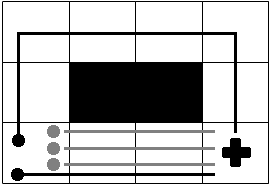
\includegraphics[width=0.48\columnwidth]{figures/unbalanced.png}
	}
	\caption{\label{unbalanced}
	     Unbalanced ambush.}
\end{figure}

The algorithm would search for the maximum ambush
rate and in case of a tie it would go for the path that
achieves the best distribution. The $\Delta$ value alone is
not enough to compare two ambush strategies.

\subsection{Complexity}

This variation of \ambush\ is more inefficient than the
original version. If $T(G,A)$ is the
complexity in time of computing \ambush\ for a graph
$G=(V,E)$ with $|A|$ agents and the number of candidates 
to be selected as radius points is $k$, the complexity
of the \sarambush\ is $\bigO(k\cdot T(G,A))$.

Since $k \in \bigO(V)$ (selecting every possible node
as radius) the worst case of the algorithm is
$\bigO(|V|\cdot T(G,A))$. Alternative candidate sets
can be constructed from taking nodes that are separated
by distances that are incremented exponentially, for
example, selecting the nodes in positions that are
powers of two in the \astar\ path ($1, 2, 4, 8, \ldots$).
This variation leads to an increment of only $\bigO(log(|V|))$.
In the following experiments the radius set contains
every node in the \astar\ path.
